\documentclass{article}
\usepackage{interspeech2006,amssymb,amsmath,epsfig}
\usepackage{hyperref} % For hyperlinks in the PDF

\usepackage{natbib} % Harvard style bib
\bibliographystyle{IEEEtranN}

\usepackage{lipsum} % Dummy text
\usepackage{listings} % Code
\usepackage{color}
\lstset{basicstyle=\ttfamily,
  showstringspaces=false,
  commentstyle=\color{red},
  keywordstyle=\color{blue}
}

\setcounter{page}{1}
\sloppy		% better line breaks
\ninept
%SM below a registered trademark definition
\def\reg{{\rm\ooalign{\hfil
     \raise.07ex\hbox{\scriptsize R}\hfil\crcr\mathhexbox20D}}}


\title{System Software: Adding System Calls to the Linux Kernel}

\makeatletter
\def\name#1{\gdef\@name{#1\\}}
\makeatother
\name{{\em Anthony Troy and Liam Allen}}

\address{School of Computing  \\
Dublin City University \\
Dublin 9, Ireland\\
{\small \tt\{anthony.troy3,liam.allen5\}@mail.dcu.ie}
}

% You should submit a brief report, maximum of 8 pages, describing how you implemented the call, details of the changes made to the system files. 
% A listing of the application program, and a C program example using it.


\begin{document}

\maketitle

\begin{abstract}
Linux is arguably the most extensible and powerful operating system in existence today. 
Now with supports for ARM, x86-64, Alpha, PowerPC, SPARC and other architectures, 
the kernel is running on everything from small consumer electronics to supercomputers.
Mainstream Linux distributions aim to serve the needs of the majority, providing
interoperability with most common hardware such as display, sound and wireless devices.
Nevertheless, the exact needs of a user are rarely met by one distribution.
Accordingly one can customise the kernel for their given environment.
These adjustments might simply involve the tweaking of kernel parameters or removing
unneeded modules. More intricate alternations include adding custom 
kernel patches and modules. 
This papers briefly reviews the 
fundamental mechanism which facilitates this
extensibility, the kernel system call interface. Subsequently, in conjunction 
with our accompanying source code, we contribute the implementation of two trivial Linux system
calls.
\end{abstract}

\section{Introduction}
Since being first developed in 1991 by Linus Torvalds, Linux has quickly 
the surpassed the hobbyist market to becoming widely adopted in 
production environments. It currently powers everything from ``cell 
phones and embedded devices to more than 90 percent of the world's top 
500 supercomputers" \citep{Love7}. Then studying at the University of Helsinki,
Torvalds was abashed by the state of the operating systems (OS) space. Dominant 
OSs at this time were either proprietary or inextensible Unix systems. 
Accordingly, Torvalds released an immature but full-fledged Unix that was extensible
by design and licence. It is important to note that the initial success of the project 
would not have been possible without this permissive open-source license. 
Not long thereafter, Linux quickly attracted interests of many and ``evolved into a collaborative 
project" \citep{Love}.
\par
Today Torvalds continues to be the principal author and maintainer of the kernel while 
being backed by a sparse group of contributors. These developers are primarily 
sponsored by corporations such as Red Hat, Intel, IBM, Texas Instruments, Google
and Samsung, though anyone can potentially contribute. Being licensed under the
``GNU General Public License (GPL) version 2.0", one can download the kernel source
code and modify it, however distributing any changes requires making the altered source 
code available \citep{Love}. 
\par
Notwithstanding its monolithic design, \citet{Kroah} asserts that the kernel is the 
most flexible OS in existence. More specifically, Linux can be characterised 
as a ``modern" monolithic kernel in that it provides a high-level interface over the hardware
but can also load executable modules at runtime. Before we explore the kernel's
system call application programming interface (API), it is important to take stock
of exactly what the kernel is responsible for in terms of the overall operating system.
\par 
Albeit an undesirable thing to do, it is indeed possible 
to run programs on a machine without a kernel. Nevertheless, the
presence of a kernel  of course ``simplifies the writing and use of other programs,
and increases the power and flexibility available to programmers" \citep{Kerrisk}.
Meaning, on a high-level, the kernel provides a layer of abstraction over a machine's 
resources. Among other things, this layer is responsible for the 
following:
\vspace{1.8mm}
\begin{itemize}
  \item \textbf{Process creation and termination.} Under Linux a process
  is a program in execution wherein the object code is loaded 
  into memory along with other resources such as ``open files and pending signals, internal kernel data, processor state, a memory address space with one or more memory mappings, one or more threads of execution, and a data section containing global variables".
   Upon creation, the kernel first ``forks" 
a copy of the parent task and then ``execs" the process by loading the new
executable into the address space Upon termination, the kernel frees any resources
held by the process and notifies the parent \citep{Love}.
 \item \textbf{Process scheduling.} The Linux kernel is preemptive and multitasking, meaning
 that the rules determining when given processes get ran and on what CPU is managed by
 a separate subsystem, the kernel scheduler.\ Information about each process is held in a
process descriptor in dynamic memory and the scheduler divides processor time 
between runnable scheduled processes \citep{Love7, Kerrisk}.
 \item \textbf{Memory management.} In terms of user-space, 
 physical memory is a limited resource which must be fairly and efficiently shared among
 processes. As Linux is a virtual memory OS, the kernel virtualises memory among processes. 
 Meaning each process conceptually ``has full access to the system's physical memory" 
 from within their own process address space \citep{Love}.
 \item \textbf{Filesystem interfacing.} Linux's Virtual Filesystem (VFS) is a kernel
 subsystem which provides filesystem-related interfaces to user-space programs. Importantly,
 ``all filesystems rely on the VFS to enable them not only to coexist, but also to interoperate"
  \citep{Love}. Hence, a single call to read a file from any filesystem on any device is made possible. 
 \newpage
 \item \textbf{Device interfacing.} Simplified through VFS, the
 kernel provides standardised APIs to interface with mounted compute devices. 
 The kernel's process scheduler also arbitrates the concurrent access of multiple
processes to each device.
\end{itemize}

\noindent Robert \citet{Love7}, a long-standing developer on the Google kernel team, 
stresses that no other OS has scaled so well while supporting so many 
hardware types and environments. These feats were made possible 
through the maintenance of a concise and fundamental interface 
from which processes interact with the system, the system call
API. The rest of this paper discusses this interface while 
contributing two example system call implementations
 

\section{System Calls} 
\subsection{Syscall Interface}
In addition to providing mechanisms to create and terminate processes, 
system calls (or syscalls) permit processes to interact with hardware 
and other OS resources. They essentially act as concise entry-points into the kernel. 
Consequently, it is important to note that, in contrast to normal user applications, 
the kernel lives in a privileged system state having a ``protected memory space and full 
access to the hardware". Whereas user-space hosts only user-defined applications that see a subset 
of the available system resources \citep{Love}. This 
bridging interface over privileged resources
is key in ensuring that processes do not misbehave, which
in turn provides a more stable system.
\par
In general applications never directly execute system calls, instead
standard C library functions are often used which in turn implement
the system call interface. For instance, the fopen() function extends upon 
the open() syscall whereby it opens the file pointed to by path string parameter and returns the
associated stream \citep{Kerrisk}. These abstractions over syscalls provide caller-friendly interfaces 
which serve to save developer time in both writing and debugging code. Other notable 
library functions implementing system calls include write(), printf(), malloc() and free().
\par
The number of calls available is architecture dependant, 
however typically more than 90 percent of syscalls are implemented by all architectures. 
Interestingly, notwithstanding its large code base, the Linux kernel only implements around 350 system 
calls as of version 3.0 \citep{Love7}. Each system call is represented by a unique number that 
cannot change. The kernel does not facilitate for the dynamic adding or removing of syscalls, in
turn syscall numbers cannot be recycled as this would break backward-compatibility. 
\par

\subsection{Syscall Invocation}
From the application perspective, a C library function implementing a 
syscall executes as transparently as any other function. On the surface 
fopen() terminates the same way strcpy() does. This is because syscalls
in Linux ``are faster than in many other operating systems" \citep{Love7}.
The kernel is quickly and transparently switching from user-mode to kernel-mode,
executing the call and returning back to user-mode. The implementation of
fopen() invokes a software interrupt to switch to kernel-space through 
incurring a special exception to be managed by the system call handler.   
\par
In Fig 1, we illustrate the high-level steps involved in invoking execve() 
under an x86-32 architecture. First, the programs invokes the library function
which involves preparing the function arguments for the kernel by placing them 
into registers on the stack. Following, the function stores the execve() system call
number in another register. Now prepared for the context switch, the function invokes
the software interrupt instruction (0x80) which prompts the system
call handler to transfer the register values onto the kernel stack. Subsequently, 
the execve() system call service routine is invoked wherein the parameter 
values are validated and the requested work is performed. Finally the 
kernel stack registers are restored and execution returns to the execve() library 
function with an integer flag to indicate the success or failure of the system call.

\begin{figure}[h]
    \centering
    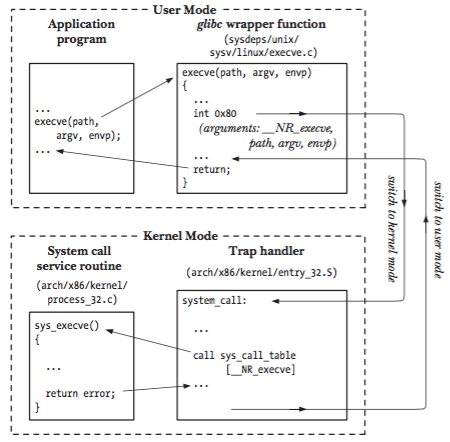
\includegraphics[width=0.462\textwidth]{img}
    \caption{Invoking a syscall (x86-32)}
    \label{fig:img}
\end{figure}


\section{Study: Adding a Syscall}

\citet{Love7} asserts that a new system call should be both purposeful and ephemeral in execution while also standing the test of time. 
Meaning that a new system call should not be multiplexing. It should have one purpose which is fulfilled efficiently and transparently 
in adherence with the Unix motto, ``provide mechanism, not policy". Accordingly, 
an overly precise interface may not fair well over time so it should be generalised where possible. 
\par
Adding a new Linux system call is relatively simply. Our accompanying source code demonstrates
how straight-forward this actually is. Nevertheless, it is important to note
that there are compelling reasons against adding 
a system call in practice, these are as follows: for most use-cases a syscall is overkill; 
after a syscall is released the interface cannot ever change;
and going forward each architecture needs to support the syscall.
\par 
We present the adding of two trivial x86-32 system calls, the first simply generates some
kernel logs and the second deals with kernel data structures. Our enclosed 
source code is in text snippets form representing the additions made to
the 3.3.8 kernel. These files are follows:
\begin{itemize}
  \item src/bootstrap.sh
  \item src/install.sh
  \item src/Makefile\_snippet.txt
  \item src/arch/x86/syscalls/syscall\_32\_snippet.txt
  \item src/include/linux/syscall\_snippet.txt
  \item src/hello/hello.c
  \item src/datastructs/datastructs.c
  \item test/userspace\_hello.c
  \item test/userspace\_datastructs.c
\end{itemize}

\subsection{Preparatory Work}

\noindent Admittedly, our selection of the 3.3.8 kernel on a Debian 6 distribution
does not have great significance. In contrast to the 2.6 series, for our purposes 
we only gain an easier to configure default boot-loader (Grub2) along with a smarter 
`make config' kernel task. The commands to fetch and prepare our kernel source
for development are captured in our bootstrap\@.sh bash script. It includes the following commands: 
\begin{lstlisting}[language=Bash]
#!bin/bash
sudo apt-get install gcc -y && \
sudo apt-get update -y && \
sudo apt-get upgrade -y && \
wget $KERNEL_SRC \
  -O linux-3.3.8.tar.xz && \
rm -fr $USER/dev && \
mkdir -p $USER/dev && \
tar -xfv linux-3.3.8.tar.xz \
  -C $USER/dev/linux-3.3.8
\end{lstlisting} 
Custom kernel sources are often mistakenly placed in the /usr/src directory. 
In practice it is strongly discouraged to develop under /usr/src/linux as it is
commonly ``the location of the kernel that 
the system libraries were built against" \citep{Love}. Accordingly, we develop
our kernel source from a user directory.
\par
Compiling and installing the Linux kernel only
requires installing the Make and GNU Compiler Collection (gcc) packages on 
most Linux distributions. As the kernel
developers use ``both ISO C99 and GNU C extensions to the C language", 
we need at least gcc version 3\@.2 but 4\@.4 onwards is recommended \citep{Love7}. 
After installing gcc 4.4.5 we fetch the kernel source tarball and move into 
our target user directory for development.
\par
Now prepared for development we can begin adding our system calls.
At runtime the kernel stores all registered system calls as function-pointers 
in the sys\_call\_table array. This list is partly derived from the given architecture's system call table; 
a declarative file which lists all the supported syscalls by number and function name. Thus,
for our purposes we append to only the syscall table for x86-32 as follows:
\begin{lstlisting}[language=Bash,  tabsize=4,
  showspaces=false,
  showstringspaces=false]
350	i386	hello	     sys_hello
351	i386	datastructs  sys_datastructs
\end{lstlisting} 
In practice a new system call should be captured in include/asm/unistd\@.h, wherein 
the new syscall call's number is mapped to a constant. Consequently, developers
do need to keep track of the actual system numbers, only the corresponding names need to be referenced
\citep{Love7}. 
For the sake of brevity and simplicity we bypass this step and later reference the syscall number explicitly.
Nevertheless, such an alternation would involve appending the following to the unistd header file:
\begin{lstlisting}[language=C]
#define __NR_hello       350
#define __NR_datastructs 351
\end{lstlisting}
Before implementing our system calls we must first define their respective
prototypes. Like any C function that needs be used across object files,
an associated prototype must be declared in a header so the
function can ultimately be linked. Regardless of corresponding target architecture, all
system call prototypes reside under the include/linux/syscall header file. Thus,
we append the following prototypes: 
\begin{lstlisting}[language=C]
asmlinkage long sys_hello(const char *test)
asmlinkage long sys_datastructs(void)
\end{lstlisting} 
Miscellaneous syscall implementations commonly live in kernel/sys\@.c which, like
all source living under the 'kernel' module, is compiled into the kernel image. Alternatively,
one can define a new module to be compiled along with the kernel.  Being adventurous, we create 
two new modules for our respective syscalls as follows:
\begin{lstlisting}[language=Bash]
#!bin/bash
cd $USER/dev/linux-3.3.8 && \
mkdir -p hello && \
touch hello/hello.c && \
echo "obj-y := hello.o" \
	>> hello/Makefile && \
mkdir -p datastructs && \
touch datastructs/datastructs.c && \
echo "obj-y := datastructs.o" \
	>> datastructs/Makefile
\end{lstlisting} 
Finally, these new modules must be added to the kernel's compilation pipeline. In defining respective
Makefiles for these modules we add their compiled object files to a "obj-y" variable, this ensures
that kbuild will include these objects files in the overall kernel build. For kbuild to first be aware that
there new modules to track we must update the primary kernel Makefile as follows:
\begin{lstlisting}[language=Bash]
core-y := usr/ hello datastructs
\end{lstlisting} 
  
\subsection{Saying Hello World}
With our preparatory work now in place we can implement our first system call which 
simply demonstrates some basic kernel logging. The involved source is as follows:
\begin{lstlisting}[language=C]
#include <linux/kernel.h>
#include <linux/syscalls.h>
asmlinkage long sys_hello(const char *test)
{
    printk(KERN_ALERT "Hello %s\n", test);	
    return 0;
}
\end{lstlisting} 

\subsection{Dealing with Kernel Data Structures}
Our second and slightly less-naive system call involves playing around task\_structs, which are circular doubly-linked lists representing processes or tasks. 
The implementation is as follows:
\begin{lstlisting}[language=C]
#include <linux/kernel.h>
#include <linux/syscalls.h>
#include <linux/printk.h>
#include <linux/sched.h>
#include <linux/thread_info.h>
#include <asm-generic/current/h>
asmlinkage long sys_datastructs(void)
{
    printk(KERN_ALERT "Current \
          process name is: %s \n", 
          current->comm);
    printk(KERN_ALERT "Current \
    	   PID: %i \n", 
	   current->pid);
    printk(KERN_ALERT "Parent \
    	   process name: %s \n",
	   current->parent->comm);
    printk(KERN_ALERT "Parent \
          process PID: %i \n", 
          current->parent->pid);
 	
    for_each_process(task)
    {
        pr_info("%s [%d] %ld %d \n", 
            task->comm, task->pid, 
            task->state, task->prio);
    }
    
    return 0;
}

\end{lstlisting} 

\subsection{Installing and Testing the Kernel}
Given that our new system calls are implemented we can begin to compile and install the kernel.
Similar to our bootstrapping script, the commands to configure and install our custom kernel
are captured in our install\@.sh script. 
It includes the following commands: 
\begin{lstlisting}[language=Bash]

#!bin/bash
cd $USER/dev/linux-3.3.8 && \
rm -f ./.config && \
sudo cp /boot/config-`uname -r` .config && \
sudo chown $USER ./config && \
yes "" | make oldconfig && \
make -j4 && \
sudo make install_modules install && \
sudo mkinitramfs \
    -o /boot/initrd.img-3.3.8 3.3.8 && \
sudo update-grub && \
sudo reboot

\end{lstlisting}   
As entailed above, we first configure and compile our new kernel. Taking our
old configuration file from the currently installed kernel we can be almost 
assured that there will be configuration parity between both kernels. Subsequently,
we install compiled kernel's binary, a vimlinux file, into the boot directory 
by running the install Make target. Similarly, we install our compiled kernel modules 
into /include/modules with by running install\_modules. Following, we must
create initramfs image corresponding with our kernel as on boot 
it will used an initial root file system. Finally, we update our boot-loader to respect 
our new linux image by making it bootable. 
Upon restarting our machine we can then boot from our custom linux 3.3.8 kernel and test our 
new system calls. A userspace program testing both calls is as follows: 
\begin{lstlisting}[language=C]



#include <unistd.h>
#include <stdlib.h>
#include <stdio.h>

int main()
{
    syscall(350, " World!");
    
    int pid;
    syscall(351);

    pid = fork();	
    if(pid < 0)
    {
        fprintf(stderr, 
                "Fork Failed \n");
	 exit (-1);
    }
    else if(pid == 0)
    {
        execlp("cat", "cat", 
               "/var/log/kern.log", NULL);
    }
    else
    {
        wait(NULL);
	printf("Child complete \n");
	exit (0);
    }
    return 0;
}
\end{lstlisting} 



\section{Conclusions}
No longer a hobbyist project,
the Linux kernel is now a powerful and interoperable operating system that is currently 
powering smartphones, supercomputers, desktops and web servers. 
Being extensible in both design and licensing it is easy 
to customise the kernel to particular needs. In this paper we reviewed 
the central interface that allows the kernel to be so flexible while remaining stable.
Linux system calls serve as a managed bridge into the kernel and must be carefully 
designed and implemented. Along with our accompanying source code, this paper
contributed a detailed implementation of two Linux syscalls,
demonstrating the approachability and simplicity of the Linux system call interface.



\vspace{-7.5mm}
\renewcommand{\refname}{\section{References}}
\bibliography{is2006_latex_template}

\end{document}
